\chapter{The \Lambdair, CPS, Codegen \& FFI}
System F IR 的繁饰标志着编译“上升期”的结束；\Lambdair\footnote{
  \Lambdair 是致敬 Appel 在其工作 \emph{Compiling with Continuations}（可能也包括 SML/NJ 编译器）使用的同名 IR；
  \Tigris 本身则是致敬 Appel 的 \emph{Modern Compiler Implementation in ML}，昵称\emph{虎书}，因为其封面有一只老虎。
  \Tigris 有拉丁语的老虎之意。
}则作为一个真正的中间表示（intermediate representation, IR），标志着编译“下降期”（降级）的开始。
\Lambdair 应当算做 ANF，后者是函数式语言编译器常用的一类 IR.

ANF 的精髓在于\emph{变量}。在 ANF 中，某一语言对象，或（非基础的，nontrivial）表达式，都由 Let-绑定捕捉为变量，
并通过后者指代：这一特性在某种程度上与汇编代码类似。虽然 \Tigris 编译到高级语言，但其后端代码风格
与手写程序不同，因而 SBCL 可以从中获得一定优势，相当于 \Tigris 编译器已经帮其做了部分工作。

\section{\Lambdair}
\paragraph{\Lambdair 的定义}
\Lambdair 的设计从六大角度开展：值、右手侧、陈述语句、尾调用位置、表达式、函数。对应到实际实现，就是
\texttt{Value}、\texttt{Rhs}、\texttt{Stmt}、\texttt{Tail}、\texttt{LExpr}、\texttt{LFun}，我们将逐一介绍
各个部分。\underline{读者应当注意上述六个类型是互递归的。}
{\setlength{\parskip}{-1em}
  \subparagraph*{\texttt{Value}} 也叫立即数/值，不能再化简。
  立即数包括变量、常量（整数、字符串、布尔值、幺元）、构造值和 Lambda 抽象。应当注意，
  此时的 Lambda 抽象还并没有经过闭包转换，因此可以捕捉自由变量。
  \subparagraph*{\texttt{Rhs}} 指 ANF 的右手侧，且只能以变量作为参数。
  右手侧包含原生函数（整数四则运算、常量的等号）、字典投影、元组、构造子应用（在定义上与立即值的构造值一致，但意义不同）、
  构造子测试（即测试两构造子是否相同）与函数调用。
  \subparagraph*{\texttt{Stmt}} 指陈述语句，目前只有 Let1.
  \subparagraph*{\texttt{Tail}} 表示尾调用位置，即某一函数的最后一条语句（一个操作）
  但不仅包括函数调用，还有函数返回、条件表达式、多分支条件匹配表达式（switch）和一特殊 token \texttt{MATCHFAIL}. \texttt{Tail} 具有标注
  尾调用位置的重要功能，方便后期做尾调用优化。在具体实现中，switch 语句又依匹配对象不同分为常量、构造值两类——这样的区分
  有利于后期更方便地做常量折叠优化。
  此外，\texttt{MATCHFAIL} 是一特殊常量，用于表示不完全模式匹配的后备分支。如前文所述，若进入这个分支，则程序立即抛出错误并终止。
  在具体实现中，其能够接收一个被匹配对象变量名的参数，后者会传递到并用于后端代码生成，以产生更好定位的错误信息。
}
\subparagraph{\texttt{LExpr} 与 \texttt{LFun}} 前者是 \Lambdair 程序的主体，包含序列操作、
立即数 Let-绑定（记 $\mathbf{let}_\iota$）、右手侧 Let-绑定（记 $\mathbf{let}$）、LetRec-绑定（记 $\mathbf{let}_\omega$）：三种 Let 因其右手侧不同而不同，
分别是 \texttt{Value}、\texttt{Rhs} 和递归定义。

\texttt{LFun} 则表示 IR 中的一个顶层函数，
是一个3-元组 \texttt{(fid, param, body)}，
分别代表函数名、参数名和函数体（\texttt{LExpr}）。
在具体实现中，LetRec-绑定携带一列顶层函数（\texttt{LFun}），而非 \mintinline{lean4}|Name × Name × LExpr|，即便
LetRec 绑定的是本地函数。原因完全是性能上的，因为两者具有相容的表示，直接使用前者替代后者能够省去两种类型之间多余的转换。

尽管 \Tigris 是纯函数式语言，我们仍用序列操作 \texttt{seq} 来捕捉尾调用 \texttt{Tail}。这是因为具体实现中，只有 \texttt{seq} 结点
能够携带尾调用信息。而且，考虑到以后可能为 \Tigris 加入不纯模式，将其转变为类似 OCaml 的语言，具备 \texttt{seq} 结点
可以减轻工作量。

\Lambdair 沿用前述的 pretty-printing 算法，但因为篇幅限制，我们不再给出范例。读者只需知道其语法类似 Haskell 和 SML 的混合体即可。

IR 降级的过程中有一些很可注意的细节。下面针对降级期间的特殊情形作探讨。

\paragraph{捷径: 构造子与原生操作}
\Tigris 的七种原生操作与0-元构造子不存在函数调用产生的性能损失，而原生调用的检测则是通过语法树上的模式匹配实现的。
因而有时需要做 $\eta$-expand，否则可能出现漏检情况。具体实现中，无论是原生操作还是普通函数，对降级过程而言都是相同的，径由
\texttt{App} 分支，但很明显特殊对待前者能够获得更好的性能——目前两者唯一的区别就是其标识符——通过在降级最开始的位置匹配这些标识符，
我们即可优先处理原生调用，避免普通调用产生的性能损失（目前编译器未做内联优化）。

\begin{minted}[numbers=left,baselinestretch=1]{lean4}
partial def lowerF (e : FExpr) (ρ : Env) (ctors : Std.HashMap String Nat)
  (k : Name -> M σ LExpr) : M σ LExpr := do
  match matchBinaryPrim e with
  | some (op, x, y) =>
    lowerF x ρ ctors fun vx =>
      lowerF y ρ ctors fun vy => do
        let r <- fresh "p"
        let cont <- k r
        return .letRhs r (.prim op #[vx, vy]) cont
  | none => (...) -- 此处处理构造子（与上同）和普通降级
\end{minted}

\paragraph{字典投影} 如前文所述，是专门为类型类方法设计的。根据最原始的字典传递实现，
方法是通过模式匹配投影出来的。这不仅增加代码生成体积，亦容易复杂化降级过程。因而我们在前文引入这一结点，并在
\Lambdair 的降级过程中传递，最后在后端直接生成投影代码，避免经过模式匹配。

\paragraph{函数，函数应用与逆柯里化}\label{sbcl:cav} 函数式语言通常保证柯里化。但当我们考虑
生成代码时，就不得不注意其带来的性能问题——为 $n$-元函数产生 $n$ 个函数显然是不现实且臃肿、低效的，同时还增加目标语言做
尾递归优化的难度。因而绝大多数以函数作为头等对象的语言（广义上的函数式语言）都做逆柯里化（uncurrying）优化。该优化通过将连续的
函数头（柯里化满足这一特征）压缩成一个 $n$-元组作为单参数（这是我们的具体实现）以便被编码为立即值 \texttt{Value} 并简化柯里化函数的 IR 降级。
有以下若干值得注意的概念：

{\bf 解构连续函数头} 是用于压缩（squash）具有连续函数头（无论是否由柯里化造成）的函数，例如 \mintinline{lean4}|fun x => fun y => ...|，
并返回 3-元组 \texttt{(p0, rest, core)}，分别指代函数首参数、剩余参数与函数体。

{\bf $\eta$-expansion} 不仅仅指 \lambdacalc 中的计算法则，在此处更指用于解决降级的函数应用（\texttt{App}）分支并未正确
处理的边界情况。考虑应用通过模式匹配投影产生的函数，如
\begin{minted}[frame=single]{ocaml}
let boxed = Boxed (_ + _) and unwrap (Boxed f) = f
in unwrap boxed 20 20
\end{minted}
其中 \texttt{unwrap boxed 20 20} 称为\emph{高阶应用}（higher-order application）：\texttt{boxed} 的应用在 Let 程序体内发生，但
并不能被降级过程捕捉，因为只有应用头 \texttt{unwrap} 对其可见，且 \texttt{unwrap} 是一高阶函数（即它返回函数，但其函数体内没有应用），
因而这条语句其实发生\emph{两次}函数应用，但降级过程只可见第一次；图 \ref{fig:higher-order} 形象地给出了两次函数应用。
\begin{figure}[H]
  \[
    \begin{tikzcd}
      {\mathsf{unwrap}} && {\mathsf{boxed}} && {20\ 20}
      \arrow[""{name=0, anchor=center, inner sep=0}, "{\text{\textcircled{\tiny 1}}}"', curve={height=-18pt}, from=1-1, to=1-3]
      \arrow["{\text{\textcircled{\tiny 2}}}", curve={height=-30pt}, Rightarrow, from=0, to=1-5]
    \end{tikzcd}
  \]
  \caption{高阶应用}\label{fig:higher-order}
\end{figure}
应用\textcircled{\scriptsize 1}对降级过程可见，但是，\underline{由其\emph{返回的函数产生的}应用\textcircled{\scriptsize 2}对降级不可见}。
因而，\texttt{unwrap}在这一过程中会 $\eta$-expand 为 \mintinline{ocaml}|let unwrap (Boxed f) x y = f x y|，显式化
高阶应用。$\eta$-expansion 过程产生的参数有 $..\eta N$ 的形式，例如 \texttt{\_pR\#η0}.
熟悉\lambdacalc 的读者或许知道 $\eta$-expansion 可能在 CBV 下带来意想不到的求值语义——譬如上文提到的
$\mathsf{Y}$ 组合子的 Church 实现若不加更改，在 CBV 下\emph{不会停机}，但 $\eta$-expansion 推翻了这一结论，
产生\emph{语义不一致}问题——且我们无法避免其发生。因此，与其无条件地做 $\eta$-expansion，我们只对
上面这种情况特殊处理，其余不变，以期尽可能减少对于语义的影响。

此外 Lean 亦有 $\eta$-expansion 导致语义不一致的问题，但由于危害不大，其开发者目前也不准备对此做任何处理。
见脚注笔者发表的 Proofexchange 帖子\footnote{\url{https://proofassistants.stackexchange.com/a/4424}}，
以及帖子中 Lean 类型论设计者的回答和 GitHub issue \texttt{\#5908}\footnote{\url{https://github.com/leanprover/lean4/issues/5908}}.

{\bf 语法元数（syntactic arity）} 指的是用户在函数定义时给出的元数。问题在于将不同种类的元数同上述的高阶应用/函数混搭时
易出现问题，而函数式语言恰巧存在大量此种风格的程序。一般来说，降级工作通过检查函数对应的类型来决定函数的元数——实践中发现这一检查并不足够。
考虑上文的 $\mathsf{unwrap} : \mathsf{BoxedAdd}\to\Int\to\Int\to\Int$，从类型上看应为 3-元函数（由于柯里化），但根据用户给出的定义，其实际上只接受一个参数——
即便传给其另外两个参数，它也不知道该怎么办——因为其函数体根本没有出现另外的参数。因而，只有在经过 $\eta$-expansion 后它才能够是真正的 3-元函数。相比于类型决定的元数，
在逆柯里化工作中，我们更多依靠语法元数。

{\bf 逆柯里化投影生成} 指的是为逆柯里化的函数生成投影代码的过程。因为我们使用元组来实现逆柯里化，因而
在函数实际要使用传入的参数时需要首先将其投影出来。这一变换通常与闭包转换一起进行，在下文介绍。

{\bf 栈底层降级工作} CPS 风格的递归代码在降级过程中是经常使用的，而递归的首要工作就是明确基准情况（base case）——续点栈（continuation stack）底层的
降级工作 \texttt{lowerFCore} 所表示的就是这一情况。\texttt{lowerFCore} 可以看作和 IR 中的 \texttt{Tail} 存在\emph{同像性}（homoiconicity）\footnote{确切的说，和第二部分提到的 \texttt{chainl/chainr} 的一致，这也是一种\emph{同态}。}，因为
从降级工作的角度，或是 IR（即 object language，数理逻辑上的\emph{对象语言}）的角度而言，两者都代表尾调用——\underline{\texttt{lowerFCore} 本身也用于 \texttt{Tail} 的降级}。
\begin{minted}[escapeinside=`',numbers=left,baselinestretch=1]{lean4}
def lowerFCore (e : FExpr) (ρ : Env) (ctors : HashMap String Nat) : M σ LExpr :=
  lowerF e ρ ctors $ pure `$\circ$' .seq #[] `$\circ$' .ret
\end{minted}
其中 $(\circ)$ 表示函数复合运算符，在函数式语言中十分常见。对比之可以发现，
栈底层的降级 \texttt{lowerF} 不需要传入续点 $k :\mathsf{Name}\to\mathsf{M}\;\sigma\;\mathsf{LExpr}$，因而不存在由续点造成的\emph{控制转移}（control transfer）。
我们将在 CPS 化一节中谈到续点、续点传递（化）的概念。

实现逆柯里化是在函数定义和函数应用上共同努力的结果——不妨先定义逆柯里化函数的参数安排（layout）。对于某 $n$-元函数的参数 $a_1,\dots,a_n$，构造 $pl$（payload）其中

\begin{equation}
  pl =
  \begin{cases}
    ((), ()) & n = 1, a_1 = ()\\
    (a_1, ()) & n = 1\\
    (a_1,\dots,a_n) & n \ge 2
  \end{cases}
\end{equation}

笔者必须承认，事后考虑起来，这一 layout 存在一些设计问题。虽然它是元组，但编码上其与 \texttt{List} 相仿，比如单元素时
在元组尾端加入了一个哨兵幺元（sentinel），但在 $n\ge 2$ 时又将之去掉。如果——且恰巧——没有类型信息的辅助，
要判断这一元组的形状较难，为后端代码生成徒增麻烦。此外，我们还应当在编译器前端就将语法元数收集起来，
而不是在这一阶段按需收集，导致代码的可维护性下降。

从函数应用的角度考虑，逆柯里化的函数在应用时必须区分\emph{完全应用}与\emph{部分应用}。我们的做法是分情况讨论：
对于前者，分为单参数、类型/语法元数不匹配两种情况进行处理；
对于后者，根据缺少的部分计算需要补充的元数，并根据数目封装一层新 Lambda 抽象。
同理，对于函数形式的值——构造子，我们也采取相同的操作。但由于构造子毕竟不是函数，
不具备函数体，仅仅是能够应用，则处理起来相对简单许多。

\paragraph{模式匹配} 是通过决策树算法\footnote{
  从实现上看，完全/冗余性检查可以看作是这一算法的超轻量版本。
}
开展编译工作的。我们定义三种类型 \texttt{Sel}、\texttt{RowState}、\texttt{DTree}，分别表示
模式投影、模式行向量以及决策树的数据结构本身。其中，决策树有五个分支，分别编码匹配失败、
叶子（即一个行向量）、常量匹配、构造子匹配与元组模式分割。在 PL 术语中，模式匹配编译工作的
目标叫做匹配自动机（matching automata），主要分为\emph{决策树}（decision tree）以及\emph{回溯自动机}（backtracking automata）。
后者较为简单，且与人的思考方式类似：从模式矩阵的左上角开始，按先行后列顺序匹配矩阵中的每一个模式，直到其到达矩阵右下角（即遍历）。
这类自动机的好处在于能够保证本部分代码生成的线性大小。但是正如其名，它可以回溯、重复匹配某些分支或模式，导致运行时的性能问题。
与之不同，我们实现了一个能够保证不存在重复匹配同一值、模式对的决策树模式匹配编译器。
为了展现这一编译器的优势，我们沿用 Maranget 工作的一个范例，考虑
（为可读性，用 \texttt{F}、\texttt{T}、$(\cdot)$ 表示 \texttt{false}、\texttt{true} 和通配符）模式矩阵
\[
  \begin{pmatrix}
    \cdot & F & T \\
    F & T & \cdot \\
    \cdot & \cdot & F \\
    \cdot & \cdot & T \\
  \end{pmatrix}\Longrightarrow
  \begin{pmatrix}
    1 \\ 2 \\ 3 \\ 4
  \end{pmatrix}
\]
在我们的实现下被翻译为（$\varnothing$ 表示后备分支或通配符分支）以下 IR：

\begin{minted}[ignorelexererrors=true,numbers=left,frame=single]{sml}
case x of
  false → case y of
            true  → case z of true → RET 2 | false → RET 2
            false → case z of true → RET 1 | false → RET 3
  ∅     → case y of
            false → case z of true → RET 1 | false → RET 3
            ∅     → case z of true → RET 4 | false → RET 3
\end{minted}

可以看出在\underline{最坏情况}下，仅需 3 次即可得出结果，相比回溯自动机快上许多。当然，我们发现
其实可以提出第 3 行的公共表达式，消去无用分支并直接返回 2. 但这已超出
决策树的优化范围且我们并没有做相关优化。不仅如此，由于在类型检查部分做过完全性检查，已经分担了
一部分决策树算法的工作，因而此处实际上实现了一个\emph{轻量}版的决策树算法，因为可以沿用
前面步骤得到的信息。

\section{\Lambdair 的闭包转换}

\paragraph{闭包转换} 指的是将本地函数提（hoist）到全局，并将之变换为全局函数的操作。
实际的工作并不像听起来一般简单，因为本地函数——其他语言常有的 lambda——会捕捉当前词法作用域内的
自由变量，因而主要挑战就是消去这些捕捉的自由变量。
虽然一些文章认为闭包转换与 lambda 提升（lifting）有差异，因为前者只是将自由变量加入参数列表而
不调整调用处——此处仍用“闭包转换”一词表示 \Tigris 取两者其中的实现思路：我们实现了前者，但同时亦
做了一些独属于后者的变换，故而称之“取两者其中”。

此外，有一些读者可能要问，既然我们以本就是函数式语言的 Common Lisp 作为编译目标，为何还要花费心思去
做这一件事——原因主要是工作量上的，我们希望重新发明轮子以展示本项目的工作量，同时亦作为一种对函数式语言
设计实现的实践训练，还为本课题的目标对象——开展编程语言实践训练的学生们作为学习样例。

\subparagraph{“中间派”闭包转换实现思路} 指我们将 \Tigris 程序中出现的所有 Lambda 都进行闭包转换，并
为之添加一个显式的\emph{环境参数}用于存储捕捉的自由变量的步骤。这一环境参数同函数指针\footnote{
  在 SBCL 后端中，“指针”无非是用来指代函数的标识符，从语义上可称指针，非 C 语言的同名概念。
}一起包装，
称为\underline{函数对象}（function object）。当我们应用函数对象时，环境参数 $\Gamma$（后同）会同逆柯里化的参数元组，即
前面的 $pl$\footnote{
  读者注意，后文用 $pl$ 指代逆柯里化的参数元组与环境参数的综合体，而非单独的前者。
}
组装起来，并一同传给函数指针。“取两者其中”体现在我们虽然消去了所有的自由变量，但同时也创建了
一个函数对象，虽然函数本身在这一过程中已经\underline{提到顶层}。而当提到（referencing，指调用或传递）该函数时，
我们实际上是在指代函数对象而非孤零零的函数指针。因而，我们不仅消灭了 lambda，也修改了函数调用位置，既不是单纯的
闭包转换，也没有完全达到 lambda lifting，因为后者不允许出现上面的 $\Gamma$.

与逆柯里化一样，闭包转换也在影响着函数定义与应用的方方面面。在介绍这两个概念后，
现在便可给出 \Tigris 的函数调用规范（function calling convention）。

\subparagraph{函数调用规范}\label{fn:calling-conv}从本质上看就是函数对象的编码。综合以上内容，\Tigris 的函数调用规范由以下四点给出：

1. $pl$ 即 payload，指经过闭包转换的函数的参数，有 $pl=\inmark{arg, \Gamma}$ 其中
$arg$ 指逆柯里化产生的参数元组。

2. $\Gamma$ 又称闭包环境，指对捕捉的自由变量的显式存储。闭包环境是一构造值 $\mathbf{E}\sem{fv_1,\dots,fv_n}$，
在实践中，为了避免构造子标识符的冲突，我们使用不能通过词法分析的特殊符号 \texttt{U+1D404 MATHEMATICAL BOLD CAPITAL E}
指代闭包环境构造子。$\Gamma$ 与其余构造值并无不同，仍然使用现有 IR 的语言组件编码。

3. \emph{闭包} 又称函数对象，是 2-元构造值 $\mathbf{C}\sem{ptr, \Gamma}$ 其中 $ptr$
指代一函数指针（又称代码指针，code pointer），指针本质上是字符串。具体实现中，为了避免构造子标识符的冲突，
我们使用不能通过词法分析的特殊符号 \texttt{U+1D402 MATHEMATICAL BOLD CAPITAL C} 指代函数对象构造子。
同上，闭包仍然由现有 IR 的语言组件编码。\emph{闭包应用}是通过投影 $pl=\inmark{arg, \Gamma}$ 并将 $(arg, \Gamma)$ 传给 $ptr$ 实现的。

4. \emph{互递归}广义上包括单递归，是通过将某一 Letrec-绑定组做变换使得其中的每一个函数的函数体都从 payload 中
投影 $(arg, \Gamma)$. 函数体内的递归调用直接使用同一个闭包环境\footnote{
  其好处在于能够避免每次递归都要组装一遍 $pl$ 带来的多余性能损失。通过这点
  我们能够获得逼近在目标语言中原生递归函数的递归性能（因为生成的后端代码的递归调用与原生无异）。
}，
一组互递归函数共享同一 $\Gamma$.

前文说过，\underline{\Tigris 不区分函数绑定与传统意义上的值绑定}，这就是说任一函数定义都可视作（也实际是）
一个 lambda 抽象——所以无论一个函数全局与否，其总是要经过闭包转换。而对所谓的全局函数而言，闭包转换就在\emph{全局}
收集自由变量并显式地存在对应的闭包环境中。这样做，保证了理论的统一性（\lambdacalc 本不存在全局/本地的差异），也
简化了代码实现，使得我们不必特殊处理全局函数。

\begin{remark}[性能考量]
  有读者可能认为对于全局定义、不包含自由变量（$\Gamma=\varnothing$）的函数来说，将其不断的装入/脱去某函数对象是一件
  很没必要且浪费性能的事情，为什么不直接应用这些函数——的确，本文作者极其认同这一点。在
  旧版的 \Tigris 中我们启用了这一试验性优化，但也因此产生了一些问题，所以目前为禁用状态。
  虽然作者同样认为占据程序性能大头的（互）递归函数才是真正的问题所在，
  而这类函数依据上面的调用规范不存在这一性能问题，因此我们认为实际性能影响并不很严重。
\end{remark}

\begin{remark}[优化：融合立即出现的尾调用]
  我们用一个简单的模式匹配来处理极常见的一种可以优化的情况：如果表达式具有模式 $f^\mathsf{T}(a)$，其中 $f$ 是上一行（层）代码刚刚由 $fid, \Gamma$ 构造的函数对象，我们将之改写为
  $fid^\mathsf{T}(\inmark{a, \Gamma})$，并通过下文将要介绍的 DCE 优化将不再用到的旧函数对象删除。
%\begin{Verbatim}[numbers=left,baselinestretch=1]
%def fuseTail (envName x fid : Name) : LExpr -> LExpr
%  | .seq binds (.app f a) =>
%    if f == x then
%      let pl := "ρ"; .seq (binds.push (.let1 pl (.mkPair a envName))) (.app fid pl)
%    else .seq binds (.app f a)
%  | .letVal y v b => .letVal y v (fuseTail envName x fid b)
%  | .letRhs y r b => -- (..同理，略..)
%\end{Verbatim}
\end{remark}

\section{\Lambdair 的优化}

\paragraph{代码优化} 是在闭包转换前后所做的。闭包转换之后可能暴露出更多优化机会、产生更多语法噪音，
因此需要重新过一遍优化。\Tigris 编译器目前主要有三种优化：常量折叠/传播、复制传播及死代码消去（dead code elimination，DCE）和
最为重要的尾调用优化（tailcall-ify）。

{\setlength{\parskip}{-1em}\subparagraph{常量折叠与传播} 指通过将绑定的常量传播到所有与之相关的代码，并在编译期
  直接计算出结果的优化。目前而言，\Tigris 编译器可以做整数的四则运算与所有常量类型的相等比较。虽然
  这里涉及的许多操作可能存在结合律、交换律与分配律，我们的实现目前\emph{不支持}这些变换。例如 $10 + 10 + x + 10$
  可以化简为 $20 + x + 10$，但并非 $30 + x$. 当然，编译器还支持控制流语句的折叠，譬如模式匹配搭配条件语句
}
\begin{minted}[frame=single]{ocaml}
let xy = {x = 1, y = 2} and b = true
in let {x = x', y = y'} = xy 
in if b then x' + y' else 0
\end{minted}
\enlargethispage{.8cm}
会被化简到 $3$. 除此之外，常量折叠搭配类型类能产生意想不到的效果。考虑某一通过变量名实现的实例，如用
整数的相等关系 \texttt{eqInt} 实现 \texttt{Eq} 的 \texttt{(=)} 方法。当我们在代码中调用后者如 \texttt{(1 = 0)} 时，
因常量折叠能够处理字典投影，表达式直接被重写为 \texttt{eqInt 1 0}. 这一优势在于传统的字典传递实现的类型类，
虽较面向对象的接口更快，但仍然存在字典投影的 overhead. 通过常量折叠，我们能真正地实现纯静态编译期的
类型类系统，达成\emph{零成本抽象}。

\subparagraph{复制传播与死代码消除} 前者与其他优化，比如上述常量折叠一同使用，通过 Let-绑定中等号的传递性，编译器能够
追逐（chase）某一标识符，直到其表示某一常量为止。沿用上例：编译器之所以知道 \texttt{xy} 指代前面的结构体，就是得益于复制传播。

另一方面，DCE 就如同其字面义一般简单：消除所有无用的代码，比如某一函数中从来未使用过的绑定。\Tigris 的问题在于其
虽然是纯函数式语言，但我们也提供了直接通过 FFI 引入副作用的 hack. 因而在新版本的 \Tigris 中 DCE 不再过于激进，
如果 Let-绑定的左手侧是一通配符模式，则我们不移除这条代码，因为这种写法常见于不纯函数式语言中用于执行某些具有副作用的代码，例如 OCaml.

\subparagraph{尾调用（tailcall）优化} 是函数式语言必备的一个优化。使用任一函数式语言或阅读过 \emph{SICP}\footnote{
  \emph{Structure and Interpretation of Computer Programs}
}的读者可能已经对此比较熟悉，但我们仍不厌其烦地在下文作一简单介绍。

函数式语言最明显的特征之一就是其在程序中广泛地使用函数\footnote{这里使用表示函数的底层意义的 subroutines 一词为宜。}。函数与调用栈（call stack）不可分割：
当程序通过某一调用进入 subroutine 时需要将对应调用的上下文（返回点、栈上分配的值）压入调用栈中。
当 subroutine 重新将控制权移交回上一级，则出栈。若某程序的栈空间用完，则其将被操作系统杀死并
产生\emph{栈溢出}异常。然而我们发现，在程序（函数）的中间调用其他函数，与在尾部
调用是两种不同的情况——后者可看作控制权的移交（transfer of control）\footnote{
  显然控制权的移交还包括各种控制流语句或非本地出口。后者指那些不是通过函数返回跳出某一函数的情况，
  例如 goto、throw 或 early return.
}，因而可用
指令 \texttt{j} 而非 \texttt{call} 替代（假设 RISC-V ISA）。相比后者，前者在控制转移后可
立即弹出栈帧，释放栈空间。称后者\emph{尾调用}。

显然，最需要调用栈资源的语言对象就是递归调用了。我们称一个函数是\emph{尾递归}（tailrec）的，当其以
调用自身（或同一互递归函数组的函数）结尾。在这种情况下，一个经过尾调用优化的函数会不停的
在尾递归调用之间压栈、出栈调用栈。\emph{尾调用优化}使得像这样的函数（包括非递归函数）的空间复杂度为 $\mathcal{O}(1)$
而非 $\mathcal{O}(n)$. 图 \ref{code:tail-comparison} 展示了两组互递归函数，一组具备尾调用优化的\emph{先决条件}，一组则不具备。
\begin{figure}
  \centering
  \begin{subfigure}{0.65\textwidth}\centering
    \begin{minted}[frame=single]{ocaml}
let rec countTree
  | Empty => 0
  | Node _ f => 1 + countForest f
and countForest
  | Nil => 0
  | Cons t f => countTree t + countForest f
    \end{minted}
    \caption{非尾递归}
  \end{subfigure}%
  \begin{subfigure}{0.35\textwidth}\centering
    \begin{minted}[frame=single]{ocaml}
let rec even
  | 0 => true
  | n => odd $ n - 1
and odd
  | 0 => false
  | n => even $ n - 1
    \end{minted}
    \caption{尾递归}
  \end{subfigure}
  \caption{}\label{code:tail-comparison}
\end{figure}

将一个函数转变为尾调用风格，既可以通过手写，也可以通过机械化的 CPS 变换（但后者性能通常相对差）。直观的说，尾递归函数在
语义和思考模式上和\emph{迭代}相似，而后者的栈空间复杂度显然是 $\mathcal{O}(1)$. 根据上面的叙述，
有读者会问：尾调用优化看似是在底层做的，那么 \Lambdair 层面的尾递归优化到底代表什么呢？

答案是我们在这一阶段\emph{标记}尾调用位置（由 \texttt{Tail} 的 \texttt{app} 构造子编码）并将这一信息传递给
后端，由其保证在生成的 LISP 代码中标记的尾调用位置不变——如果缺少这一信息，后端的压力会大上许多。上面说过，
尾调用位置形如 $f(arg)^\mathsf{T}$，其中 \texttt{f} 根据编译阶段是（CC 前后）函数名或函数指针。简单总结
几个优化的顺序，就是
\begin{align*}
  \text{\circled{1}\ 常量折叠} && \text{\circled{2}\ DCE} && \text{\circled{3}\ 尾调用标记} && \text{\circled{4}\ DCE}.
\end{align*}

最后，用于总结这一部分的内容，我们来探讨上文反复提到的 \underbar{CPS}，
亦为下一部分续点传递化的叙述作理论基础。CPS 作为一种编程风格，在我们的降级实现中十分常见。
续点函数（continuation function）$k$，由同像性，
在对象语言中表示一个\underline{挖\ruby{空}{kòng}}（pluggable）的表达式，即从这一点往后的程序。
\begin{figure}[htb]
  \[
    \begin{tikzcd}[column sep=small,row sep=scriptsize]
      {k:} & {\mathsf{Name}} && {M\ \sigma\ \mathsf{LExpr}} &&& {\text{（元语言；仅含类型）}} \\
      \\
      {\mathbf{let}} & {[\bullet]} & {=\cdots\ \mathbf{in}} & e &&& {\text{（对象语言：\Lambdair）}}
      \arrow[from=1-2, to=1-4]
      \arrow["{\text{plugging}}", from=1-2, to=3-2]
      \arrow["{\text{lowering}}"', from=1-4, to=3-4]
  \end{tikzcd}\]
  \caption{CPS 化在元语言与对象语言间的同态}\label{fig:cps-homoicon}
\end{figure}

挖出的“空” $(\bullet)$ 应当（若有意义）在 $e$ 中有引用。我们称之“挖空”，是因为如同
“填空题”一般，将这一续点应用（把空填上）到某个语言对象（这里只能是变量，即字符串）上，比如变量 $m$，则会使得 $m$ 在 $e$ 中有绑定，
\underline{并返回\emph{剩余}表达式，即该点往后的程序}；图 \ref{fig:cps-homoicon} 形象地展示了这个性质。
从这个意义上讲，续点可以看作是一个程序的\emph{模板}。从实现的角度考虑，这不过是在显式的 CPS 栈\footnote{CPS 栈本身既存在于元语言（实现），亦存在于对象语言 \Tigris.}中运行单子 $M$ 下的操作而已——
CPS 栈是我们显式维护的，本质上是由许多用于降级工作的小续点（续点在编程语言中基本使用函数编码，除非原生支持）\emph{复合}而成的大闭包；
使用 CPS 风格实现递归，根据上述同态我们能够轻易地在元语言（即 Lean）中传播对象语言（即 IR）中的变量。

\paragraph{增量式 API 与 \emph{Tigrisi} IR 解释器} 是本项目编程子系统的一个试验性扩展。
虽然 \Tigris 的编译器 \texttt{tigrisl} 能一遍直接完成从源代码到可执行程序的产生，这样的编译管线却
不适用于 REPL，因为两者在编译过程上有着不同的使用逻辑和性能要求：用户使用交互式的 REPL 时通常\emph{一步步地}输入程序，
但又希望在每一次输入后能立马得到当前的结果。一个最直接的 REPL 可能只是
缓存用户到目前为止输入的所有程序，并在每一次输入之后重新编译\emph{整个程序}——对于具有多阶段的
语言实现来说效率极其低下，尤其是当程序较大时，越往后的输入就需越多无用的重新编译。因而，我们编写了
一套试验性质的增量 API，用于\emph{增量编译}：用户输入一部分程序，我们就编译一部分；从不重新编译已经
编译过的部分。

实现增量编译，重点在于记录编译器每个阶段出现的状态——将用户上一次输入时的\emph{所有状态}，
传递给下一次输入的编译过程即可
——难点在于，虽然纯函数式编程通过单子或最基本的函数传参实现
显式的状态管理与可预见的副作用管理，各个编译阶段仍然存在不少的中间（临时）状态，这些状态并不通过函数返回、
且在对应编译过程结束后消失，造成 API 设计的困难。因为这套 API 并未经过全面测试且实现简单，
可认为其是试验性的。由此出发，我们实现了 \texttt{tigrisi} IR 解释器，以 \Lambdair
作为解释对象。

\subparagraph{\emph{Tigrisi} 解释器} 严格说来，可以独立于增量 API 运行。
虽然启用增量 API 能带来更好的编译期性能——解释器本身是稳定的。下面介绍这一解释器的设计。

解释器，如同虚拟机（virtual machine）或物理机一般，存在\emph{状态}。例如 OCaml VM 能够运行 \texttt{ocamlc}
输出的字节码，是因为其存在一全局状态。广泛地说，需要这些状态是因为绝大多数编程语言都存在绑定这一语法结构，无论全局/本地，
或是函数式与否。因而，状态本质上是一个映射，或键值对构成的表（例如哈希表或树表）。设计解释器一个重要的性能考量是想办法
将这些状态做得\emph{轻量}。作为数据结构来说，分配/投影/修改这些状态都需要时间与空间。

我们定义解释器的状态为：由哈希表编码的，字符串（变量）到立即数的映射。
而此处的立即数则包含函数指针、所有的常量、
元组、构造值且后两种结构亦只能由立即数组成。
\emph{Tigrisi} 解释器的状态有三种，分别记录本地绑定、全局绑定与函数绑定。

\enlargethispage{\baselineskip}

当遇到一个 \texttt{let*}\footnote{
  此处的 \texttt{*} 指通配符，可以匹配空字符串、$\iota$ 或 $\omega$，与 \Lambdair pretty-printed 的
  语法一致。和 LISP 或 OCaml 的序列绑定没有任何关系。
}，其携带的绑定会按类型插入到上述任一表中。此外，解释器还运行在 \texttt{EIO}（带 I/O 与错误处理副作用的单子）中，
且支持多线程：求值过程独立运行于一个线程中，这使得用户能够通过快捷键 \texttt{<C-c>} 来终止
当前求值线程。在 Lean 中线程的终止是需要合作实现的，并非只要用户请求，线程就一定会被杀死，需要线程本身作出回应。
\begin{wrapfigure}{l}{0cm}
  \centering
  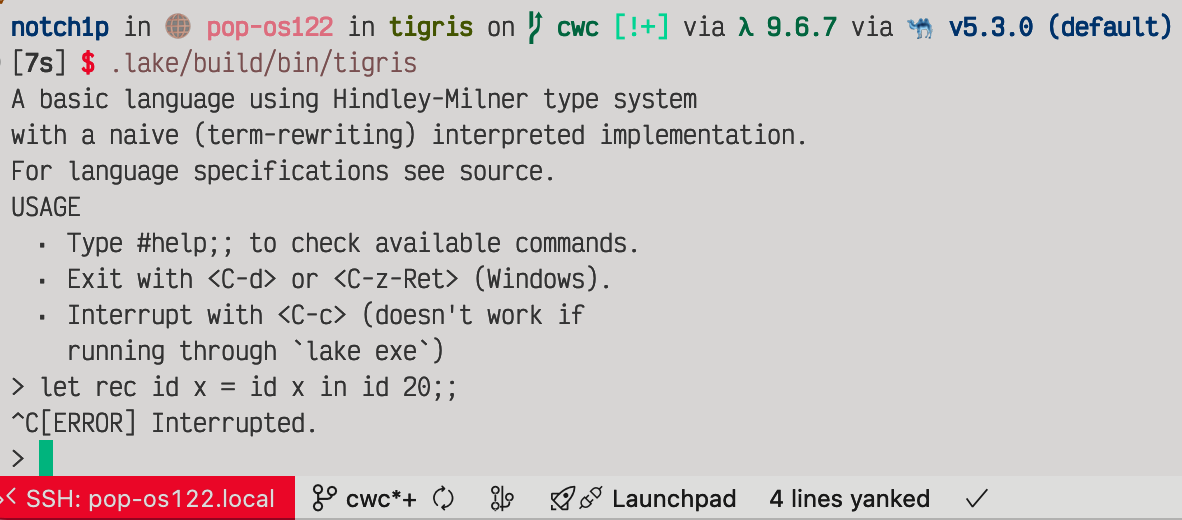
\includegraphics[width=0.38\linewidth]{assets/term1}
  \caption{某用户终止一次计算}\label{img:term1}
  \vspace{-1em}
\end{wrapfigure}
我们通过在解释器的热点分支之前做线程终止检测，以回应来自用户的线程终止信号，并在收到信号的同时跳出函数，实现
线程的正常终止。而之所以能够通过 CLI 前端按快捷键终止线程，是程序通过 Lean 的 C FFI 初始化
POSIX SIGINT 管道，捕捉用户发出的中断信号并提供管道的读写方法实现的。同时，我们还在 Lean 侧设置
一\emph{哨兵线程}，不断读取管道值以检测信号是否发出，若发出则终止。
\begin{minted}[numbers=left,baselinestretch=1]{c}
typedef lean_obj_res OBJRES; static int32_t sig_pipe[2] = {-1, -1};
LEAN_EXPORT OBJRES lean_sigint_pipe() {
  struct sigaction sa;
  if (sig_pipe[0] != -1) return lean_io_result_mk_ok(lean_box(sig_pipe[0]));
  if (pipe(sig_pipe) != 0)
    return lean_mk_io_user_error(lean_mk_string(/* ..错误信息.. */));
  memset(&sa, 0, sizeof(sa)); sa.sa_handler = sigint_handler;
  sigemptyset(&sa.sa_mask); sa.sa_flags = SA_RESTART;
  if (sigaction(SIGINT, &sa, NULL) != 0) {
    close(sig_pipe[0]); close(sig_pipe[1]);
    sig_pipe[0] = sig_pipe[1] = -1;
    return lean_mk_io_user_error(lean_mk_string(/* ..错误信息.. */)); }
  return lean_io_result_mk_ok(lean_box(sig_pipe[0])); }
\end{minted}
而这整套机制，由状态 \texttt{EvalState} 记录，
\begin{minted}[numbers=left,baselinestretch=1]{lean4}
abbrev EvalState := Option $ Task $ Except Error 
                  $ REPLState × LInterpreter.Val × Scheme
\end{minted}
其中 \texttt{Task} 是 Lean 原生类型，表示异步计算，与协程（coroutine）相仿，例如 Scala 的 \texttt{Future}，JS 的 \texttt{Promise} 和 Rust 的 \texttt{JoinHandle}.
总的来说，\emph{Tigrisi} 的实现是多方努力的成果：Lean 侧与 C 侧通过 FFI 实现中断机制的底层；
REPL 前端与解释器协作实现用户输入、编译器前端处理与降级、解释器求值与输出、出错中断、手动中断这一循环。

现在，若某程序不停机或运算时间过长，例如 \mintinline{ocaml}|let rec loop x = loop x in loop ()|，用户
即可通过快捷键 \texttt{<C-c>} 终止对应线程，如图 \ref{img:term1} 所展示的那样。
\emph{Tigrisi} 的主要功用并非
运行程序，而是方便开发者能够快速判断编译器的 IR 降级阶段是否实现出错。

\section{CPS 化}
\paragraph{CPS\upcite{reynolds1972definitional,sussman1998scheme} 变换} 亦称 CPS 化，指将 \Lambdair 转变为 CPS 风格 IR 的变换过程。以我们的实现为例，
CPS 变换后的 IR 具备以下特征：
所有函数接受一显式续点参数 $k$；
函数调用返回的结果应当传给续点，而非直接返回；
续点\emph{并非}头等公民，必须通过本地绑定产生，或上述的续点参数 $k$. 任一函数
从不能独立返回续点本身；
前述的 ANF 特征仍保留。

在尾调用优化一节我们曾提到过 CPS 可以用于将非尾调用函数变换成尾调用——这实际上是一个很具体且片面的说法。
全面地说，机械化（即编译器所作的，而非程序员手动的）的 CPS 变换的目的是\underline{编码复杂控制流}，
类似 C 语言的 \texttt{longjmp}. CPS 变换能够以堆空间为代价，显式化控制流交接，因为续点通常
以 lambda 编码\footnote{
  后者主要在堆上分配。虽然大多数编译器也会将其优化成栈上分配，如果条件允许——虽然这么做
  相当于抵消了用 CPS 来节约栈空间的目的。
}，并与其他参数一起在函数间相互传递。一言以蔽之，
CPS 通过在堆上复合续点，以堆空间换取栈空间。而复合而成的“大续点”则可以看作一个能够
替代调用栈但位于堆上的\emph{续点栈}，后者在被应用时会（在思想上）不断出栈，释放堆空间。

CPS IR 在定义上与 \Lambdair 相仿，但为了满足续点传递风格的需求新增、修改了一些语言构件。
在尾调用 \texttt{CTail} 中，我们增加新的构造子用于表示 CPS 风格的函数应用（\texttt{appFun}），
与续点应用（\texttt{appKont}），后者在 Reynolds 的论文中又称为 APPLY 操作；统一了
立即数与右手侧，统称 \texttt{CRhs}；并在表达式 \texttt{CExpr} 中统一了不同种类的 Let-绑定，
同时新增了专门用于绑定续点的 \texttt{letKont} 构造子。而相较于 \texttt{LFun}，\texttt{CFun}
用于表示 CPS 下的函数，自然也新增了一个栏位 \texttt{kontParam} 用于记录续点参数 $k$.
此外，我们还引入一个新的指令 \texttt{halt}，但并不常用——因为在 SBCL 下程序运行完不会终止，
控制权交移 SBCL，我们可以在此基础上继续编写 LISP 代码并使用 \Tigris 程序的计算结果。

CPS 变换是 IR 降级的最后一步，此后将由 SBCL 后端直接降级到 Common Lisp.
在不考虑后端的情况下，编译产物的程序的语义与 CPS IR 的语义应该一致。
为了能够使用 CPS IR 考察 \Tigris 的操作性语义，
我们下面给出 CPS 变换的指称语义\footnote{
  对于不熟悉 PLT 的用户来说，可以将这一步看成是 CPS 变换的变换法则，指导着
  具体实现。
}，与 CPS IR 自身的指称语义。首先给出 \Lambdair、CPS IR 的形式文法。
\begingroup\allowdisplaybreaks\setlength{\abovedisplayskip}{3pt}\setlength{\belowdisplayskip}{3pt}
%\begin{align*}
%\end{align*}
\begin{equation}\label{eq:lambda-cps-formal}
  \begin{aligned}
    v \in \Val &::= x \mid k \mid \ctor(t, \bar{x}) \mid \lambda p.\, e \\[4pt]
    r \in \mathsf{Rhs} &::= \prim(\mathit{op}, \bar{x}) \mid \proj(x, i) \mid \mkpair(x, y) \mid \mkctor(t, \bar{x}) \mid \isctor(x, t, n) \mid f(a) \\[4pt]
    s \in \mathsf{Stmt} &::= \letone x = r \\[4pt]
    \tau \in \mathsf{Tail} &::=\mathbf{ret}\, x \mid f(a)^{\mathsf{T}} \mid \fail \\
    &\mid \mathbf{if}\, c\, \mathbf{then}\, e_1\, \mathbf{else}\, e_2\\[-2pt]
    &\mid \switch^{\Const}(x, \overline{k_i \to e_i}, e_?) \\[-2pt]
    &\mid \switch^{\ctor}(x, \overline{(t_i, n_i) \to e_i}, e_?) \\[4pt]
    e \in \mathsf{LExpr} &::=\bar{s};\, \tau \mid \mathbf{let}_\iota\, x = v\, \mathbf{in}\, e
    \mid \letone x = r\, \mathbf{in}\, e\\
    &\mid \letRec\, \overline{f_i(p_i) = e_i}\, \mathbf{in}\, e\\[4pt]
    r_c \in \mathsf{CRhs} &::=\prim(\mathit{op}, \bar{x}) \mid \proj(x, i) \mid \mkpair(x, y) \mid \mkctor(t, \bar{x}) \mid \isctor(x, t, n) \mid k \mid x\\[4pt]
    e_c \in \mathsf{CExpr} &::=\mathsf{tail}\, \tau_c
    \mid\letone x = r_c\, \mathbf{in}\, e_c
    \mid \letK\, \kappa(p) = e_c\, \mathbf{in}\, e_c\\
    &\mid \letRec\, \overline{f_i(p_i, k_i) = e_i}\, \mathbf{in}\, e_c\\[4pt]
    \tau_c \in \mathsf{CTail} &::=f(p, k) \mid k(v) \mid \halt(v)
    \mid \fail\\
    &\mid  \ite(c, e_1, e_2) \\[-2pt]
    &\mid \switch^{\Const}(x, \overline{k_i \to e_i}, e_?) \\[-2pt]
    &\mid \switch^{\ctor}(x, \overline{(t_i, n_i) \to e_i}, e_?)
  \end{aligned}
\end{equation}
并定义语义域（domain of semantics，可看作数据类型）为，\footnote{
  $(+)$ 和 $(\times)$ 即分别为上文介绍过的 categorical product/coproduct.
}
\endgroup
\begingroup
\setlength{\abovedisplayskip}{3pt}\setlength{\belowdisplayskip}{3pt}
\begin{equation}\label{eq:cps-sem-domain}
  \begin{aligned}
    \Val &= \unit + \mathsf{Int} + \mathsf{Bool} + \mathsf{String} + (\Val \times \Val) + (\Name \times \Val^*) + \Name \\
    \Env &= \Name \rightharpoonup \Val \\
    \FunTab &= \Name \rightharpoonup (\Name \times \Name \times \mathsf{CExpr}) \\
    \KontTab &= \Name \rightharpoonup (\Name \times \mathsf{CExpr}) \\
    \mathsf{Ans} &= \Val + \mathsf{Error}
  \end{aligned}
\end{equation}
\endgroup
变换法则 $\mathcal{C} :  \mathsf{LExpr} \to \mathsf{CExpr}$ 是在给定\emph{当前续点} $k$ 下
定义的，$k$ 应当是一个指代续点的变量，或恒等续点（函数）$\mathrm{id}_\mathsf{Ans}$，
后者仅限于顶层，且为 SBCL 后端的标准入口点。

下面，我们给出这一变换的指称语义。注意 $\mathcal{C}^k_{[\bullet]}$ 表示 $k$ 绑定的、挖空的变换法则，下标的空
表示输入域元素 $[\bullet]$，为以下之一：$v, r, s, \tau, e$，而 $\mathcal{C}^k_s\sem{\bullet}(e_c)$ 携带（thread）$e_c$.
此外，我们简单化 \texttt{let*}、\texttt{switch*} 为单绑定/匹配对象，可类推多个。
\begingroup\setlength{\abovedisplayskip}{3pt}\setlength{\belowdisplayskip}{3pt}
\allowdisplaybreaks
\begin{align*}
  \mathcal{C}_v\sem{x} &= x \tag{Values} \\
  \mathcal{C}_v\sem{k} &= \mathsf{const}(k) \\
  \mathcal{C}_v\sem{\ctor(t, \bar{x})} &= \mkctor(t, \bar{x})\\
  \mathcal{C}_r\sem{\prim(\mathit{op}, \bar{x})} &= \prim(\mathit{op}, \bar{x}) \tag{Rhs} \\
  \mathcal{C}_r\sem{\proj(x, i)} &= \proj(x, i) \\
  \mathcal{C}_r\sem{\mkpair(x, y)} &= \mkpair(x, y) \\
  \mathcal{C}_r\sem{\mkctor(t, \bar{x})} &= \mkctor(t, \bar{x}) \\
  \mathcal{C}_r\sem{\isctor(x, t, n)} &= \isctor(x, t, n) \\
  \mathcal{C}_r\sem{f(a)} &= \text{（见下方函数调用变换）}\\
  \mathcal{C}_\tau^k\sem{\mathbf{ret}\, x} &= \mathsf{tail}\, k(x) \tag{Tails} \\[6pt]
  \mathcal{C}_\tau^k\sem{f(a)^{\mathsf{T}}} &= \mathsf{tail}\, f(a, k) \\[6pt]
  \mathcal{C}_\tau^k\sem{\mathbf{if}\, c\, \mathbf{then}\, e_1\, \mathbf{else}\, e_2} &=
  \mathsf{tail}\, \ite(c, \mathcal{C}^k\sem{e_1}, \mathcal{C}^k\sem{e_2}) \\[6pt]
  \mathcal{C}_\tau^k\sem{\switch^{\Const}(x, \overline{k_i \to e_i}, e_?)} &=
  \mathsf{tail}\, \switch^{\Const}(x, \overline{k_i \to \mathcal{C}^k\sem{e_i}}, \mathcal{C}^k\sem{e_?}) \\[6pt]
  \mathcal{C}_\tau^k\sem{\switch^{\ctor}(x, \overline{(t_i, n_i) \to e_i}, e_?)} &=
  \mathsf{tail}\, \switch^{\ctor}(x, \overline{(t_i, n_i) \to \mathcal{C}^k\sem{e_i}}, \mathcal{C}^k\sem{e_?}) \\[6pt]
  \mathcal{C}_\tau^k\sem{\fail} &= \mathsf{tail}\, \fail\\
  \mathcal{C}_s^k\sem{\bar{s};\, \tau} &= \mathcal{C}_s^k\sem{\bar{s}}(\mathcal{C}_\tau^k\sem{\tau}) \tag{Stmt} \\
  \mathcal{C}_s^k\sem{\epsilon}(e_c) &= e_c \\
  \mathcal{C}_s^k\sem{(\letone x = r); \bar{s}}(e_c) &=
  \begin{cases}
    \letK\, \kappa(x) = \mathcal{C}_s^k\sem{\bar{s}}(e_c)\, \mathbf{in}\, \mathsf{tail}\, f(a, \kappa)
    & r = f(a) \\
    \letone x = \mathcal{C}_r\sem{r}\, \mathbf{in}\, \mathcal{C}_s^k\sem{\bar{s}}(e_c)
    & \text{otherwise}
  \end{cases}\\
  \mathcal{C}^k\sem{\mathbf{let}_\iota\, x = v\, \mathbf{in}\, e} &=
  \letone x = \mathcal{C}_v\sem{v}\, \mathbf{in}\, \mathcal{C}^k\sem{e} \tag{letVal} \\
  \mathcal{C}^k\sem{\letone x = f(a)\, \mathbf{in}\, e} &=
  \letK\, \kappa(x) = \mathcal{C}^k\sem{e}\, \mathbf{in}\, \mathsf{tail}\, f(a, \kappa) \tag{letRhs} \\
  \mathcal{C}^k\sem{\letone x = r\, \mathbf{in}\, e} &=
  \letone x = \mathcal{C}_r\sem{r}\, \mathbf{in}\, \mathcal{C}^k\sem{e}
  \quad (r \neq f(a)) \\
  \mathcal{C}^k\sem{\letRec\, f(p) = e_f\, \mathbf{in}\, e} &=
  \letRec\, f(p, k_f) = \mathcal{C}^{k_f}\sem{e_f}\, \mathbf{in}\, \mathcal{C}^k\sem{e} \tag{letRhs}
\end{align*}
\endgroup
最后，我们给出 CPS IR 本身的指称语义，由以下两变换给定：
\begingroup
\begin{equation}
  \begin{aligned}
    \mathcal{E} &: (\mathsf{CExpr}\oplus\mathsf{CTail}) \to \Env \to \FunTab \to \KontTab \to (\Val \to \mathsf{Ans}) \to \mathsf{Ans}\\
    \mathcal{R} &: \mathsf{CExpr}\to\Env\to\Val
  \end{aligned}
\end{equation}
\endgroup
其中第五个参数 $\Val\to\Ans$ 是外层（顶层）续点 $\mu$，亦称元续点（metacontinuation），表示
能够使该续点层级的函数返回（无论有多深）。
记 $\rho[n\mapsto v]$ 为绑定（映射）$n\mapsto v$ 到 $\rho$ 的插入操作，
具有如下语义：若键 $m$ 存在及其对应值存在，用值 $v$ 替换之。注意此处所用 $\rho,n,v$ 都是元变量；
$\mathcal{E}$ 接受一 sum/coproduct type $\mathsf{CExpr}\oplus\mathsf{CTail}$，
表示这一参数既可以是尾调用 $\mathsf{CExpr}$，也可以是表达式 $\mathsf{CTail}$.
\begingroup\allowdisplaybreaks
\begin{align*}
  \footnotemark\mathcal{R}\sem{\prim(\mathit{op}, \bar{x})}\Env &= \delta(\mathit{op}, \Env(\bar{x})) \tag{CRhs} \\
  \mathcal{R}\sem{\proj(x, i)}\Env &= \pi_i(\Env(x)) \\
  \mathcal{R}\sem{\mkpair(x, y)}\Env &= (\Env(x), \Env(y)) \\
  \mathcal{R}\sem{\mkctor(t, \bar{x})}\Env &= (t, \Env(\bar{x})) \\
  \mathcal{R}\sem{\isctor(x, t, n)}\Env &=
  \begin{cases}
    \mathsf{true} & \Env(x) = (t, \bar{v}) \land |\bar{v}| = n \\
    \mathsf{false} & \text{otherwise}
  \end{cases} \\
  \mathcal{R}\sem{\mathsf{const}(k)}\Env &= k \\
  \mathcal{R}\sem{\mathsf{alias}(y)}\Env &= \Env(y)\\
  \mathcal{E}\sem{f(p, k)}\Env\FunTab\KontTab\mu &=
  \begin{cases}
    \mathcal{E}\sem{e_f}\Env'\FunTab'\KontTab'\mu
    & \FunTab(f) = (p_f, k_f, e_f) \tag{funapp} \\
    \mathsf{Error} & \text{otherwise}
  \end{cases}\\
  \text{where}\quad\Env' &= \{p_f \mapsto \Env(p),\, k_f \mapsto \Env(k)\}, \\[-4pt]
  \FunTab' &= \FunTab, \KontTab' = \varnothing \quad \text{（本地绑定的续点不逸出）}\\[-4pt]
  \footnotemark\mathcal{E}\sem{\kappa(v)}\Env\FunTab\KontTab\mu &=
  \begin{cases}
    \mathcal{E}\sem{e_\kappa}\Env[p_\kappa \mapsto \Env(v)]\FunTab\KontTab\mu
    & \KontTab(\kappa) = (p_\kappa, e_\kappa) \tag{kontapp} \\
    \mu(\Env(v))
    & \kappa = k_{\mathsf{param}} \\
    \mathsf{Error} & \text{otherwise}
  \end{cases}\\
  \mathcal{E}\sem{\halt(v)}\Env\FunTab\KontTab\mu &= \Env(v) \tag{halt}\\
  \mathcal{E}\sem{\ite(c, e_1, e_2)}\Env\FunTab\KontTab\mu &=
  \begin{cases}
    \mathcal{E}\sem{e_1}\Env\FunTab\KontTab\mu & \Env(c) = \mathsf{true} \tag{conditional} \\
    \mathcal{E}\sem{e_2}\Env\FunTab\KontTab\mu & \text{otherwise}
  \end{cases}\\
  \mathcal{E}\sem{\switch^{\Const}(x, \overline{k_i \to e_i}, e_?)}\Env\FunTab\KontTab\mu &=
  \begin{cases}
    \mathcal{E}\sem{e_j}\Env\FunTab\KontTab\mu
    & \exists j.\, \Env(x) = k_j \tag{const switch} \\
    \mathcal{E}\sem{e_? }\Env\FunTab\KontTab\mu
    & \forall i.\, \Env(x) \neq k_i \land e_? \ \text{exists} \\
    \mathsf{Error} & \text{otherwise}
  \end{cases}\\
  \mathcal{E}\sem{\switch^{\ctor}(x, \overline{(t_i, n_i) \to e_i}, e_?)}\Env\FunTab\KontTab\mu &=
  \begin{cases}
    \mathcal{E}\sem{e_j}\Env\FunTab\KontTab\mu
    & \Env(x) = (t_j, \bar{v}) \land |\bar{v}| = n_j \tag{ctor switch} \\
    \mathcal{E}\sem{e_?}\Env\FunTab\KontTab\mu
    & \text{no match}; e_?\ \text{exists} \\
    \mathsf{Error} & \text{otherwise}
  \end{cases}\\
  \mathcal{E}\sem{\fail}\Env\FunTab\KontTab\mu &= \texttt{MATCH-FAILURE} \tag{matchfail}\\
  \mathcal{E}\sem{\letone x = r\, \mathbf{in}\, e}\Env\FunTab\KontTab\mu &=
  \mathcal{E}\sem{e}\Env[x \mapsto \mathcal{R}\sem{r}\Env]\FunTab\KontTab\mu \tag{let1}\\
  \footnotemark\mathcal{E}\sem{\letK\, \kappa(p) = e_\kappa\, \mathbf{in}\, e}\Env\FunTab\KontTab\mu &=
  \mathcal{E}\sem{e}\Env\FunTab\KontTab[\kappa \mapsto (p, e_\kappa)]\mu \tag{letKont}\\
  \mathcal{E}\sem{\letRec\, f(p, k_f) = e_f\, \mathbf{in}\, e}\Env\FunTab\KontTab\mu &=
  \mathcal{E}\sem{e}\Env\FunTab[f \mapsto (p, k_f, e_f)]\KontTab\mu \tag{letRec}\\
  \mathcal{E}\sem{\mathsf{tail}\, \tau}\Env\FunTab\KontTab\mu &=
  \mathcal{E}\sem{\tau}\Env\FunTab\KontTab\mu \tag{tail}
\end{align*}
\endgroup
受过训练的读者可以立马反应出上述 CPS IR 的一些特征，我们列在下面。

\addtocounter{footnote}{-2}
\footnotetext{$\delta$ 指原生操作；$\pi_i$ 指投影。}
\stepcounter{footnote}
\footnotetext{情况二处理顶层续点 $\mu$，相当于从当前函数返回。}
\stepcounter{footnote}
\footnotetext{注意续点自身不构成值（是二等公民）；续点由单独的续点表 $\KontTab$ 记录。}

\begin{remark}[二等公民续点] 指在本 IR 中续点只能出现在下列语法位置：
  在函数调用的第二个参数上 $f(p, k)$；
  在续点应用中 $\kappa(v)$；
  由 $\letK\, \kappa(p) = e\, \mathbf{in}\, \ldots$ 绑定
  这一性质由 CPS IR 的定义保证，因为 \texttt{CRhs} 根本不含续点（也就是说，本 CPS IR 不能返回续点）。

  有一些读者可能感到失望，因为他们发现这样的 IR 不支持更高端的原生控制流操作，例如著名的 $\mathsf{call/cc}$ 和 delimited
  continuation\upcite{felleisen1988theory} 中的 $\mathsf{shift}$/$\mathsf{reset}$. 虽然必须承认将这些操作原生化以允许
  编译器对待之能获得更好的运行时性能，但 CPS 本身并非常用的编程风格，且以程序员心智负担代价换来的
  表达力是否值得亦是需要探讨并经过调查研究的问题。我们建议即便必须使用 CPS，也应考虑 \texttt{Monad} 接口提供的\emph{内化}（internalized）的 \texttt{Cont} 单子，
  最小化 CPS 在全局的影响，并提供更好的可维护性\footnote{
    从思考难度上讲，CPS 并不直观，且滥用之与 \texttt{goto} 无异。
  }，参照 \texttt{Control.Monad.Cont}.
\end{remark}

\begin{remark}[尾调用保证] 指 CPS IR 中的任一函数调用都在尾调用位置。
  在 \Lambdair 中的非尾调用是通过 $\letK$ 编码的：
  \begingroup\setlength{\abovedisplayskip}{5pt}\setlength{\belowdisplayskip}{5pt}
  \begin{equation}
    \letone x = f(a)\, \mathbf{in}\, e
    \quad\leadsto\quad
    \letK\, \kappa(x) = \mathcal{C}^k\sem{e}\, \mathbf{in}\, \mathsf{tail}\, f(a, \kappa)
  \end{equation}
  \endgroup
  其中续点 $\kappa$ 捕捉了\underline{程序的剩余部分} $e$.
\end{remark}
%\begin{remark}[CPS 变换后的闭包表示]
%  前文我们曾介绍过函数对象的编码与调用规范——这些标准在 CPS IR 中几乎一致。考虑
%  \(
%    \mathbf{C}\llbracket \mathit{ptr}, \Gamma \rrbracket
%  \)，
%  在 CPS IR 中，函数调用变为（$p$ 仍然是前文的 payload）
%  \[
%    \mathcal{E}\sem{f(p, k)} = \cdots\ \text{其中}\ f\ \text{是一函数指针}.
%  \]
%\end{remark}
%\begin{remark}[CPS IR 模块语义]
%虽然 \Tigris 没有提供任何的模块管理功能，但其已经具备一些先决条件，譬如 CPS 变换模块中已经定义了\emph{模块}——
%任一 \Tigris 源文件自动构成一个模块。CPS IR 的一个模块包含
%  \begin{equation}
%    \begin{aligned}
%      M = (\bar{F}, F_{\mathit{main}}) && F = (f, p, k, e)\\
%      \mathcal{M}\sem{(\bar{F}, F_{\mathit{main}})} =
%    \mathcal{E}\sem{e_{\mathit{main}}}\Env_0\FunTab_0\varnothing\,\mathrm{id}_\mathsf{Ans}
%    \end{aligned}
%  \end{equation}
%  其中
%  \begin{equation}
%    \begin{aligned}
%      \FunTab_0 &= \{f_i \mapsto (p_i, k_i, e_i) \mid F_i\ \mathbf{of}\ (f_i, p_i, k_i, \cdot) \in \bar{F}\} \cup \{f_{\mathit{main}} \mapsto (p_m, k_m, e_m)\} \\
%      \Env_0 &= \{p_m \mapsto (\unit, \mathbf{E}\llbracket\rrbracket)\}
%    \end{aligned}
%  \end{equation}
%  默认的初始 payload，即 main 函数的参数为 $(((), ()), \mathbf{E}\llbracket\rrbracket)$\footnote{
%    回忆，对参数为 $a$ 的 1-元函数，我们构造 $(a, ())$ 即便 $a = ()$.
%  }，这一默认值可以轻易修改。
%\end{remark}

\section{后端: Common Lisp (SBCL) 与 FFI}\label{sect:ffi}
在进行介绍之前，不妨通过对应的数据类型先回忆一下 \Tigris 实现的所有阶段。
\begin{align*}
  \text{\Tigris 源代码}
  \xrightarrow{\text{\textcircled{\tiny 1}}}\mathsf{Expr}
  \xrightarrow{\text{\textcircled{\tiny 2}}}\mathsf{TExpr}
  \xrightarrow{\text{\textcircled{\tiny 3}}}\mathsf{FExpr}
  \xrightarrow{\text{\textcircled{\tiny 4}}}\mathsf{LExpr}
  \xrightarrow{\text{\textcircled{\tiny 5}}}\mathsf{CExpr}
  \xrightarrow{\text{\textcircled{\tiny 6}}}\text{LISP source}\\
  \text{其中}
  \begin{matrix*}[l]
    &\text{\textcircled{\scriptsize 1}}:\text{词法、句法分析}
    &\text{\textcircled{\scriptsize 2}}:\text{类型检查}
    &\text{\textcircled{\scriptsize 3}}:\text{SysF IR 繁饰、实例解析}\\
    &\text{\textcircled{\scriptsize 4}}:\text{\Lambdair 降级}
    &\text{\textcircled{\scriptsize 5}}:\text{CPS 化}
    &\text{\textcircled{\scriptsize 6}}:\text{SBCL 目标代码生成}
  \end{matrix*}
\end{align*}

\paragraph{SBCL 后端} 直接将 CPS IR 翻译为 Common Lisp 目标代码。由于 SBCL 是动态类型的函数式语言，
且 LISP 家族的语言可以直接看作无类型\lambdacalc（untyped \textasciitilde, UTLC），
多态特殊化或大部分的类型信息都不必要且续点直接由 lambda 编码，不存在任何形式的\emph{去函数化}（defunctionalization）。
选择 Common Lisp 而不是其他语言（如 JS）的原因纯粹是笔者的个人偏好，因为其喜欢使用宏。
下面非正式地给出各语言构件的直接翻译。
\begingroup\setlength{\parskip}{-.5em}
\subparagraph*{顶层函数} 指所有的函数（因为经过闭包转换）。函数 $fid(pl, k)$ 对应 \mintinline{lisp}|(defun fid (pl k))|.
\subparagraph*{Let/Kont 绑定与 kontapp} Let 绑定，即 \texttt{let1}，对应 \mintinline{lisp}|(let ((n v)) ..)|；
Kont 绑定指续点绑定，形如 \texttt{letKont k v = ..}，对应 \mintinline{lisp}{(labels ((k (v) ..)) body)}；
kontapp 指续点应用，形如 \texttt{APPLY k v}，对应 \mintinline{lisp}|(funcall (the function k) v)|.
\subparagraph*{闭包与函数调用} 闭包形如 $\mathbf{C}\sem{ptr, \Gamma}$，对应 \mintinline{lisp}|#'ptr| 若 $ptr$ 为顶层或 LISP \texttt{label} 语句绑定，
否则按构造值直接存储；闭包环境 $\Gamma$ 即 $\mathbf{E}\sem{\bar{f}}$，对每一栏位 $f$，
\begin{itemize}\itemsep-.5em
  \item 直接存储之，若其为闭包（即上述构造值），
    \item 以 \mintinline{lisp}|#'f| 引用之，若 $f$ 为顶层或 LISP \texttt{label} 语句绑定，
  \item 否则直接存储之。
\end{itemize}

函数调用形如 $f(a, k)$，对应 \mintinline{lisp}|(funcall (the function f) ..)|，如 $f$ 是本地函数指针；或 \mintinline{lisp}|(funcall #'f ..)|，如 $f$ 为顶层或 LISP \texttt{label} 语句绑定。
可以看出，函数定义、调用的形式都是一一对应的，这也符合我们的直观认识。
\subparagraph*{条件表达式与 switch 语句} 条件表达式形如 $\ite(c,t,e)$，对应 \mintinline{lisp}|(if c t e)|；
构造子匹配，形如 $\isctor(x, tag, \cdot)$，对应 \mintinline{lisp}|(eq (car x) tag)|；
switch 语句，按构造子/常量，分为
\begin{itemize}\itemsep-.8em
  \item $\switch^{\Const}(x, \overline{k_i \to e_i}, e_?)$ 对应
    \mintinline{lisp}|(cond (((equal x k_i) e_i) .. (t e_?)) ..)|
  \item $\switch^{\ctor}(x, \overline{(t_i, n_i) \to e_i}, e_?)$ 对应
    \mintinline{lisp}|(cond (((eq x t_i) e_i) .. (t e_?)) ..)|
\end{itemize}
{\setlength{\parskip}{-1em}
  \subparagraph*{元组与构造值} 元组形如 $pr = (p, q)$，对应 \mintinline{lisp}|(cons p q)|，并通过标准的
  \mintinline{lisp}|(car pp)|、\mintinline{lisp}|(cdr pp)| 投影；构造值形如 $ctag\sem{\overline{fld}}$，对应
  \mintinline{lisp}|(cons tag (vector @fld))|\footnote{
    其中 \texttt{vector} 表示 \mintinline{lisp}|'simple-vector|，即 LISP 自带数据结构中最快的连续型数组。
  }，而其投影 $x_i$ 对应 \mintinline{lisp}|(svref (cdr x) i)|. 上述特殊构造子 $\mathbf{E}$、$\mathbf{C}$ 的值亦
按此翻译。}
\endgroup

此外，出现在 CPS IR 中的所有符号，根据 LISP 的语法用 \texttt{||} 保持大小写区别。符号即对应变量——小节 \ref{sbcl:cav} 曾提到过
因为类型信息已经擦除，我们只能通过按需收集\emph{形状}来缓解歧义问题：
任何变量的初始形状都是未知的，但随着翻译进行，有可能被精练为其他形状。
由于这一做法是函数层级的，没有考虑跨函数层级的精练，且没有解决根本问题即笔者的设计失误，所以最终只能够缓解问题。
如果要从根本上解决，就必须重构降级、CPS 化，使得类型信息在经过这些阶段后能传递到后端。
\paragraph{运行时系统} 指原生操作的实现、入口代码和底层异常定义，譬如字符串等号 \texttt{\%string=}
和 \texttt{MATCH-FAILURE} 条件\footnote{
  Common Lisp 有\emph{条件系统}，较之其他语言的异常系统更加强大且泛化，因为
  可以用这一系统编码各种控制流，甚至还可以用之实现一套续点机制。
}，
在底层分别通过 SBCL 的 \mintinline{lisp}{sb-kernel:%sp-string=} 和 \mintinline{lisp}{define-condition} 实现、定义。
  Common Lisp 针对不同的数据类型有各种各样的等号。为了减少 LISP 因为动态语言产生的 overhead，我们依照表 \ref{tab:lisp-eq} 针对不同类型使用各自最适合的等号。
  \begin{wraptable}{l}{4cm}\vspace{-.6cm}\centering\caption{LISP 等号}\label{tab:lisp-eq}
    \vspace{-.3cm}
    \footnotesize
    \begin{tabular}{@{}ll@{}}
      \toprule
      \textbf{对象} & \textbf{等号}                               \\ \midrule
      Symbols/NIL/T               & \texttt{EQ}                                         \\
      Precise numbers               & \texttt{EQL}                                        \\
      Cons/String                 & \texttt{EQUAL}                                      \\ \bottomrule
    \end{tabular}
    \vspace{-.6cm}
  \end{wraptable}
  \texttt{EQ} 是物理等号，而非结构等号，即它
  比较内存地址，因而速度最快。例如在 Lean 中，构造子由整数编码，比较构造子就是比较整数——
  因为 LISP 支持符号计算，在此处构造子就是符号，由于符号在 LISP 中唯一，我们用 \texttt{EQ} 比较其
  内存地址最快，媲美 Lean 在这一步的性能。

  \paragraph{FFI} 即外部函数接口，指用于调用外部函数的语言机制。因为我们编译到 SBCL，一个
  既高层又底层的语言\footnote{
    Common Lisp 的高层在于其有垃圾回收内存管理（GC），是动态类型语言；
    其底层在于有许多可与 C 媲美且更底层的控制流操作符，例如
    \mintinline{lisp}{go}、\mintinline{lisp}{block}、\mintinline{lisp}{progn}，其历史可
    追溯到上世纪五十年代。
  }，FFI 机制已经自动成型，只要用户清楚上文介绍的函数调用规范即可。这是因为我们不必关心内存管理问题，
  或是值的 boxing/unboxing 问题\footnote{即决定一个值是立即数还是通过指针引用的问题。此处的指针就是底层的内存指针。}。
  此外，我们还活用 LISP 的元编程能力，化简 FFI 函数的定义过程，方便用户使用。
  当然，因为 \Tigris 编译器看不见也看不懂 FFI 函数的定义，因此其全盘信任用户，后者应\underline{确保 FFI 函数在 LISP 侧的名字正确、具有正确的类型声明}。

  显然，以这种方式声明的类型签名（模式）没有办法检查其正确性，也就是说，可以
  引入一些类型明显为空的值，或者那些只有通过循环论证（不停机递归函数）才能证明的类型，
  例如 $\forall\alpha.\;\alpha$ 或 $\forall\alpha,\beta.\;\alpha\to\beta$.
  当然，后者并不是毫无用处。考虑一个特殊化的版本 $\forall\alpha.\;\mathsf{Unit}\to\alpha$，
  在之后的一个例子中就能用上。
  此外，从证明论的角度考虑，一个外部函数声明其实就是一条\emph{公理}——因为我们直接声明某一个类型存在值，
  却不给出证明——这就是公理化（axiomatic）的。

  下面以一个稍复杂的例子说明 FFI 的设计和使用。首先利用 FFI 声明引入数个外部函数 \texttt{println}、\texttt{toString}、\texttt{read}，
  用于对象字符串化、stdin 输入与 stdout 输出，
  同时通过用户自定义算符引入中缀左结合 \texttt{(++)}、前缀 \texttt{(!)} 算符并将之分别绑定为字符串连接和
  即将定义的阶乘函数，即

\begin{minted}[frame=single]{lean4}
extern println  "%println"   : forall a, a -> Unit
extern toString "%to-string" : forall a, a -> String
extern read     "%read"      : forall a, Unit -> a
infixl  65  "++" => append
postfix 50  "!"  => fact
\end{minted}
  以此可实现一简单程序：用户输入一整数，打印其阶乘值及阶乘的各步骤。
\begin{minted}[frame=single]{ocaml}
let fact n =
  let rec go acc
    | 0 => acc
    | m =>
      let _ = println
            $ "fact " ++ toString (n - m) ++ " = " ++ toString (acc * m)
      in go an @@ m - 1
  in go 1 n
let main =
  let _ = println "Enter a number:"
  and x = read () in x !
\end{minted}
  因为 \texttt{x!} 也是合法标识符，所以我们用空格隔开。
  此外，\texttt{read} 不安全，因为其应用值可被实例化到任意类型，此处为 \texttt{Int}.
  具体实现中，与 FFI 定义相关联的标识符在句法分析期间就被替换为字符串内的符号，例如
  \texttt{read} 到 \texttt{\%read}. 而这几个外部函数在 LISP 侧的实现极为简单；右侧给出输出结果。
  \begin{figure}[H]\centering
    \begin{subfigure}[c]{.65\textwidth}\centering
    \begin{minted}[frame=single]{lisp}
(defforeign "%string-append" (x y)
  (declare (ignore gamma) (type string x y))
  (funcall k (concatenate 'string x y)))
(defforeign |%read| (_ __)
  (declare (ignore gamma _ __))
  (funcall k (read)))
\end{minted}
    \end{subfigure}%
    \begin{subfigure}[c]{.35\textwidth}\centering
\begin{Verbatim}[baselinestretch=1]
$ ./dist-fact.fasl
  Enter a number:
  > 5           ; stdin
  fact 0 = 5    ; stdout
  (.. 略 ..)
  fact 4 = 120
\end{Verbatim}
    \end{subfigure}
  \end{figure}
  \texttt{defforeign} 是一自定义宏，活用 LISP 元编程功能简化 FFI 函数的定义，有语法\footnote{
    读者只需要理解为：宏 \mintinline{lisp}|(defforeign function-name (x y) forms)|
    声明并返回一闭包对象，其中 \texttt{(x y)} 是 \texttt{ffi-lambda-list}，表示
    声明的函数参数，长度不定；\texttt{forms} 表示由多个语句组成的函数体。
    此处依 LISP 惯例，使用与 X3J13/CLtL2 相同的 BNF 语法。
  }
  \begingroup\setlength{\abovedisplayskip}{3pt}\setlength{\belowdisplayskip}{3pt}
  \begin{equation}
    \mathbf{defforeign}\ \textit{function-name}\ \textit{ffi-lambda-list}\ \{\textit{form}\}^*\longrightarrow \textit{closure-object}
  \end{equation}
  \endgroup
  其本质上是 LISP 函数声明与全局变量声明的结合体。
\begin{minted}[numbers=left,baselinestretch=1]{lisp}
(let* ((ns     (name-to-string name))
       (fn-sym (intern (escape-bar ns)))
       (cell   (intern ns))
       (clos   (make-closure fn-sym)))
  `(eval-when (:compile-toplevel :load-toplevel :execute)
     (defun ,fn-sym (payload k) 
                    (with-args payload ,arg-list ,@body))
     (defparameter ,cell ,clos)))
\end{minted}
  通过宏的帮助，在 LISP 侧定义 \Tigris 的 FFI 函数就和定义普通 LISP 函数一般简单。
  \section{本章小结}
  本章从 \Lambdair 及其周边、CPS 化、SBCL 后端、运行时系统与 FFI 的顺序对 Tigris 编译器的中后部分的实现与设计进行叙述，
  与实现顺序、编译顺序一致。在实现上，本章是任务最为繁重的一个模块：其不仅代表着“编译”的字面义，
  更因为本章 \Lambdair 的设计失误而加重。